\section{Definition of a photovoltaic panel model}
The last component of the simulated system is the photovoltaic panel: for this it has been needed to generate a table correlating panel's output power and input irradiation with the output current given to its load. The \emph{solar.m} file gives information about the relationship between voltage and irradiance and the output current. 

As the photovoltaic panel has a critical current over which the output power descends quickly, values over these points have been cut in order to avoid a non-invertible behaviour: as it is needed to have the current as an output value for a function, it can't be that 2 different currents correspond to the same power and irradiance. In other terms, the $(I,P)$ curve must be invertible and thus \emph{monotonic}.

With this premise, data coming from \emph{solar.m} have been used together with sample data for irradiance (\emph{example\_variable\_set.mat}) and with a sample set of voltages (in the range $[0;0.65]$), to generate and analyze the lookup table for the $I(G,P)$ power. Units have been ported to IS ones in order to avoid confusion.

The output graph is as expected: in particular, it can be seen that the maximum power that the panel can accept depends almost linearly with the input irradiance. This is a good assumption, as by fixing the area the irradiance is proportional to the absorbed power of the panel, and thus proportional to its maximum output power.

\begin{figure}[h]
  \centering
  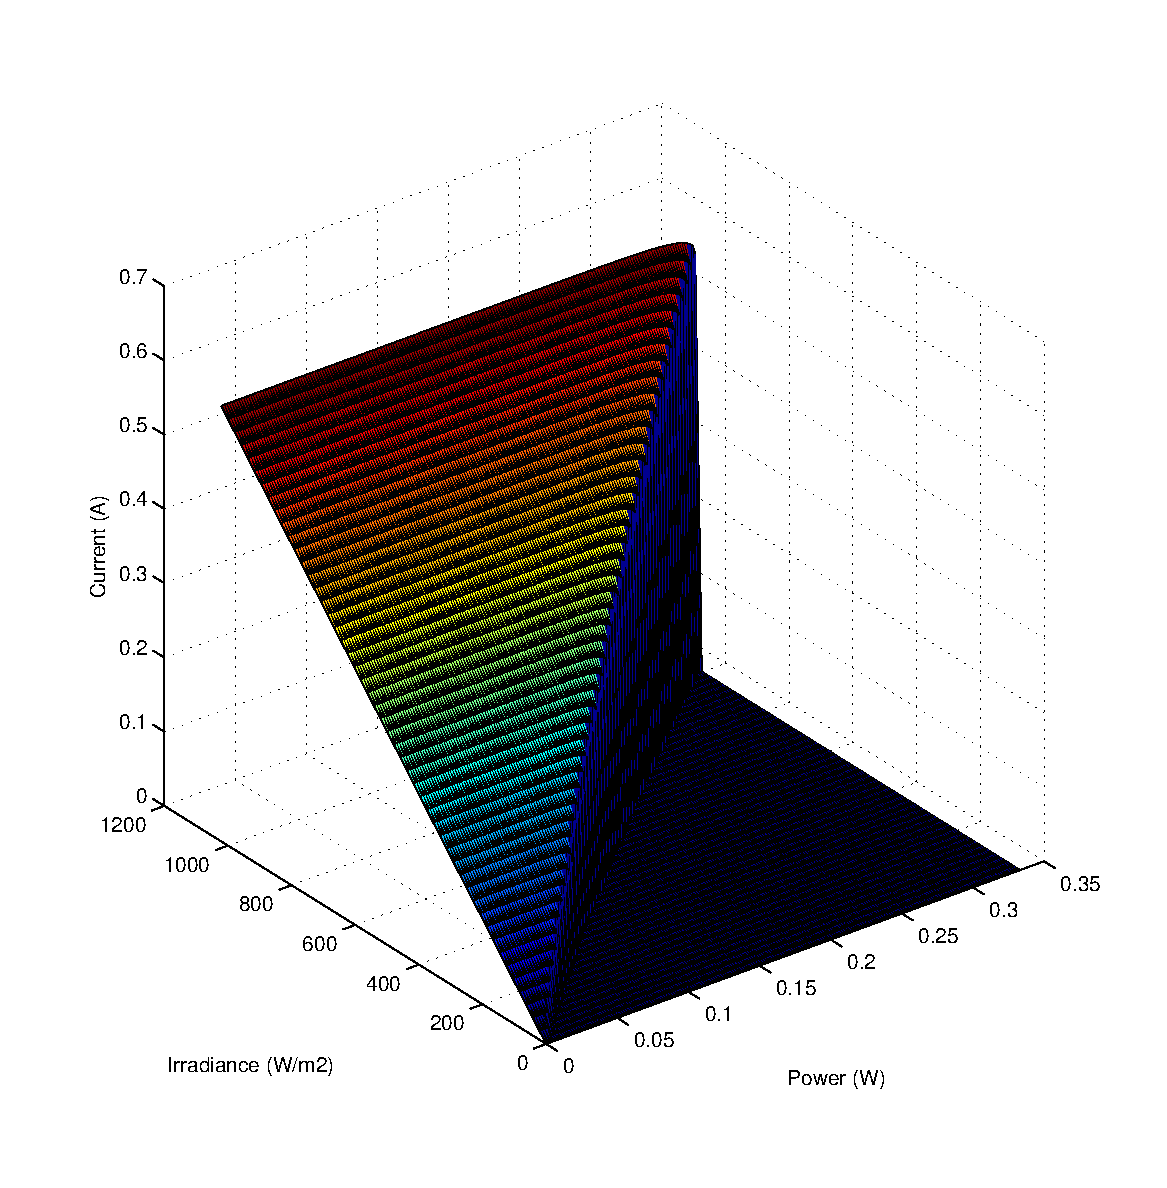
\includegraphics[width=5in]{power_irradiance_current}
  \caption{Obtained Power-Irradiance-Current surface}
\end{figure}
